\documentclass[a4paper,11pt]{extarticle}
\usepackage[a4paper]{geometry}
\geometry{verbose,tmargin=2cm,bmargin=2cm,lmargin=2cm,rmargin=2cm}

\usepackage{fontspec}
\setmonofont{FreeMono}

\setlength{\parindent}{0cm}
\setlength{\parskip}{0.5em}

\usepackage{textcomp}

\usepackage{hyperref}
\usepackage{url}
\usepackage{xcolor}

\usepackage{minted}
\newminted{python}{breaklines,fontsize=\small}
\newminted{text}{breaklines,fontsize=\small}

\definecolor{mintedbg}{rgb}{0.95,0.95,0.95}
\usepackage{mdframed}

\BeforeBeginEnvironment{minted}{\begin{mdframed}[backgroundcolor=mintedbg]}
\AfterEndEnvironment{minted}{\end{mdframed}}

\title{
MI3103 \\
Pengenalan Protokol HTTP}
\author{Fadjar Fathurrahman}
\date{2018}

\begin{document}
\maketitle

HTTP adalah singkatan dari Hypertext Transfer Protocol. HTTP merupakan protokol
jaringan tingkat aplikasi untuk sistem informasi terdistribusi, kolaboratif,
dan hypermedia. Protokol ini merupakan fondasi bagi komunikasi data untuk
World Wide Web (W3, internet) sejak tahun 1990. HTTP juga
dapat digunakan untuk keperluan selain World Wide Web.
HTTP dispesifikasikan dalam RFC-2616, yang mendefinisikan protokol yang
dikenal sekarang sebagai HTTP/1.1, yang merupakan revisi dari HTTP awal
(HTTP/1.0). Perbedaan penting antara HTTP/1.1 dan HTTP/1.0 adalah HTTP/1.0
menggunakan koneksi baru untuk tiap pertukaran permintaan (\textit{request})
dan respon (\textit{response}), sedangkan pada HTTP/1.1 satu koneksi
dapat digunakan untuk pertukaran lebih dari satu
\textit{request}/\textit{response}.

HTTP adalah protokol komunikasi yang berbasis TCP/IP, yang digunakan
untuk mengirimkan data seperti file HTML, CSS, Javascript, gambar, dan
sebagainya melalui Web.
Port default untuk protokol TCP adalah 80, meskipun port lain juga dapat
digunakan.
HTTP menyediakan cara standard bagi komputer untuk berkomunikasi
satu dengan yang lainnya.
HTTP menspesifikasikan bagaimanan data permintaan
dari klien dibangung dan dikirimkan ke server, serta bagaimana
server merespon permintaan tersebut.

Fitur dasar HTTP:
\begin{itemize}
\item Connectionless: Klien HTTP menginisiasi permintaan HTTP dan setelah itu klien
melepas koneksi dengan server dan menunggu respon dari server. Proses server
menerima permintaan dan membangun kembali koneksi dengan klien untuk
mengirimkan respon.
\item Media-independent: tipe data apapun dapat dikirimkan melalui HTTP asalkan
klien dan server mengetahui bagaimana cara menangani data tersebut.
\item Stateless: As mentioned above, HTTP is connectionless and it
is a direct result of HTTP being a stateless protocol.
The server and client are aware of each other only during a
current request. Afterwards, both of them forget about each other.
Due to this nature of the protocol, neither the client nor the
browser can retain information between different requests across the web pages.
\end{itemize}

    HTTP/1.0 uses a new connection for each request/response exchange, where as HTTP/1.1 connection may be used for one or more request/response exchanges.

Basic Architecture

The following diagram shows a very basic architecture of a web application and
depicts where HTTP sits:

HTTP Architecture

{\centering
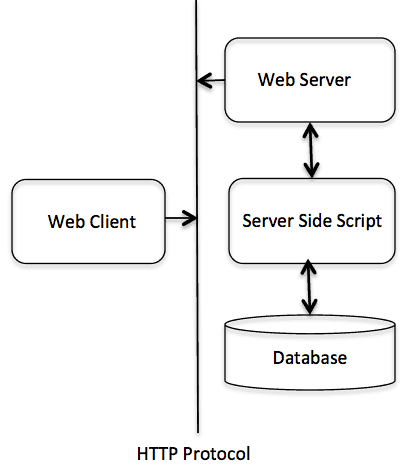
\includegraphics[scale=1.0]{images/cgiarch.png}
}

The HTTP protocol is a request/response protocol based on the client/server based architecture 
where web browsers, robots and search engines, etc. act like HTTP clients, and the Web server 
acts as a server.

Client

The HTTP client sends a request to the server in the form of a request method, URI, and protocol 
version, followed by a MIME-like message containing request modifiers, client information, and 
possible body content over a TCP/IP connection.

Server

The HTTP server responds with a status line, including the message's protocol version and a 
success or error code, followed by a MIME-like message containing server information, entity meta 
information, and possible entity-body content.

\end{document}
